% Metódy inžinierskej práce

\documentclass[10pt,twoside,slovak,a4paper]{article}

\usepackage[slovak]{babel}
%\usepackage[T1]{fontenc}
\usepackage[IL2]{fontenc} % lepšia sadzba písmena Ľ než v T1
\usepackage[utf8]{inputenc}
\usepackage{graphicx}
\usepackage{url} % príkaz \url na formátovanie URL
\usepackage{hyperref} % odkazy v texte budú aktívne (pri niektorých triedach dokumentov spôsobuje posun textu)
\usepackage{pdfpages}
\usepackage{cite}
%\usepackage{times}

\pagestyle{headings}

\title{Nový spôsob vzdelávania pomocou fenoménov\thanks{Semestrálny projekt v predmete Metódy inžinierskej práce, ak. rok 2020/21, vedenie: Mgr. Martin Sabo, PhD.}} % meno a priezvisko vyučujúceho na cvičeniach

\author{Rastislav Brna\\[2pt]
	{\small Slovenská technická univerzita v Bratislave}\\
	{\small Fakulta informatiky a informačných technológií}\\
	{\small \texttt{xbrna@stuba.sk}}
	}

\date{\small 30. september 2020} % upravte



\begin{document}

\maketitle

\begin{abstract}
	Fínsko, krajina ktorá patrí medzi lídrov vo vzdelávaní sa v rokoch 2016 - 2017 plne prešla na
	„Phenomenon-based learning”, ktoré nahradilo nám známe predmety ako matematika,
	fyzika, dejepis, atd., veľkými témami ktoré sú preberané z každej strany. Ku príkladu Druhá
	svetová vojna na ktorú sa môžeme pozrieť či už z geografického hladiska - kde všade po
	svete reálne prebiehala, historického, fyzikálneho, psychologického - mentalita ľudí v tej
	dobe/stituácii.  Je týmto spôsobom jednoduchšie učiť sa o veciach keď je vidno prepojenia
	medzi nimi ako učit sa fakty z učebnice naspamäť? Je prechod na takýto systém reálne
	zlepšením alebo sú osvedčené predmety lepšie? Prechod celého štátu na takýto systém a
	prípadné problémy.\cite{Coplien:MPD}\cite{Czarnecki:Progress}\cite{Czarnecki:Staged}\cite{Kang:FODA}\cite{PLP-Framework}
\end{abstract}



\section{Úvod}

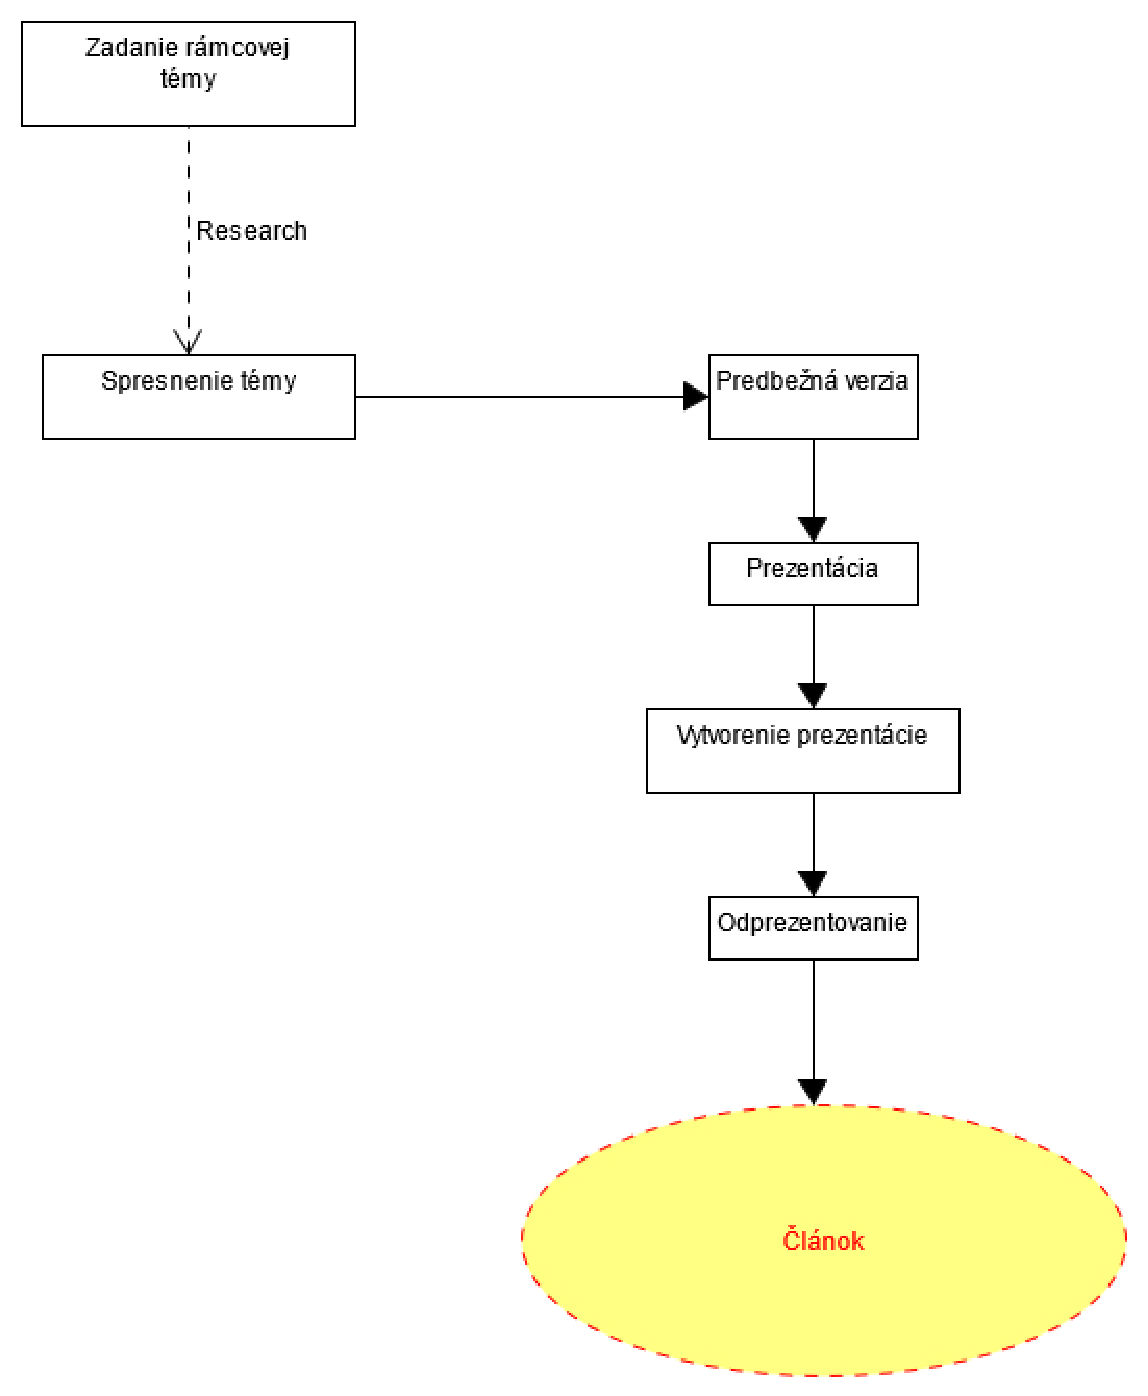
\includepdf[pages=-]{Diagram.pdf}


\section{Nejaká časť} \label{nejaka}




\section{Iná časť} \label{ina}




\section{Záver} \label{zaver} % prípadne iný variant názvu



%\acknowledgement{Ak niekomu chcete poďakovať\ldots}


% týmto sa generuje zoznam literatúry z obsahu súboru literatura.bib podľa toho, na čo sa v článku odkazujete
\bibliography{literatura}
\bibliographystyle{plain} % prípadne alpha, abbrv alebo hociktorý iný
\end{document}
